% Generated by Sphinx.
\def\sphinxdocclass{report}
\documentclass[letterpaper,10pt,openany,oneside]{sphinxmanual}
\usepackage[utf8]{inputenc}
\DeclareUnicodeCharacter{00A0}{\nobreakspace}
\usepackage[T1]{fontenc}
\usepackage[english]{babel}
\usepackage{times}
\usepackage[Bjarne]{fncychap}
\usepackage{longtable}
\usepackage{sphinx}
\usepackage{multirow}


\title{Drug Design in Parallel}
\date{July 08, 2016}
\release{}
\author{CSinParallel Project}
\newcommand{\sphinxlogo}{}
\renewcommand{\releasename}{}
\makeindex

\makeatletter
\def\PYG@reset{\let\PYG@it=\relax \let\PYG@bf=\relax%
    \let\PYG@ul=\relax \let\PYG@tc=\relax%
    \let\PYG@bc=\relax \let\PYG@ff=\relax}
\def\PYG@tok#1{\csname PYG@tok@#1\endcsname}
\def\PYG@toks#1+{\ifx\relax#1\empty\else%
    \PYG@tok{#1}\expandafter\PYG@toks\fi}
\def\PYG@do#1{\PYG@bc{\PYG@tc{\PYG@ul{%
    \PYG@it{\PYG@bf{\PYG@ff{#1}}}}}}}
\def\PYG#1#2{\PYG@reset\PYG@toks#1+\relax+\PYG@do{#2}}

\expandafter\def\csname PYG@tok@gd\endcsname{\def\PYG@tc##1{\textcolor[rgb]{0.63,0.00,0.00}{##1}}}
\expandafter\def\csname PYG@tok@gu\endcsname{\let\PYG@bf=\textbf\def\PYG@tc##1{\textcolor[rgb]{0.50,0.00,0.50}{##1}}}
\expandafter\def\csname PYG@tok@gt\endcsname{\def\PYG@tc##1{\textcolor[rgb]{0.00,0.25,0.82}{##1}}}
\expandafter\def\csname PYG@tok@gs\endcsname{\let\PYG@bf=\textbf}
\expandafter\def\csname PYG@tok@gr\endcsname{\def\PYG@tc##1{\textcolor[rgb]{1.00,0.00,0.00}{##1}}}
\expandafter\def\csname PYG@tok@cm\endcsname{\let\PYG@it=\textit\def\PYG@tc##1{\textcolor[rgb]{0.25,0.50,0.56}{##1}}}
\expandafter\def\csname PYG@tok@vg\endcsname{\def\PYG@tc##1{\textcolor[rgb]{0.73,0.38,0.84}{##1}}}
\expandafter\def\csname PYG@tok@m\endcsname{\def\PYG@tc##1{\textcolor[rgb]{0.13,0.50,0.31}{##1}}}
\expandafter\def\csname PYG@tok@mh\endcsname{\def\PYG@tc##1{\textcolor[rgb]{0.13,0.50,0.31}{##1}}}
\expandafter\def\csname PYG@tok@cs\endcsname{\def\PYG@tc##1{\textcolor[rgb]{0.25,0.50,0.56}{##1}}\def\PYG@bc##1{\setlength{\fboxsep}{0pt}\colorbox[rgb]{1.00,0.94,0.94}{\strut ##1}}}
\expandafter\def\csname PYG@tok@ge\endcsname{\let\PYG@it=\textit}
\expandafter\def\csname PYG@tok@vc\endcsname{\def\PYG@tc##1{\textcolor[rgb]{0.73,0.38,0.84}{##1}}}
\expandafter\def\csname PYG@tok@il\endcsname{\def\PYG@tc##1{\textcolor[rgb]{0.13,0.50,0.31}{##1}}}
\expandafter\def\csname PYG@tok@go\endcsname{\def\PYG@tc##1{\textcolor[rgb]{0.19,0.19,0.19}{##1}}}
\expandafter\def\csname PYG@tok@cp\endcsname{\def\PYG@tc##1{\textcolor[rgb]{0.00,0.44,0.13}{##1}}}
\expandafter\def\csname PYG@tok@gi\endcsname{\def\PYG@tc##1{\textcolor[rgb]{0.00,0.63,0.00}{##1}}}
\expandafter\def\csname PYG@tok@gh\endcsname{\let\PYG@bf=\textbf\def\PYG@tc##1{\textcolor[rgb]{0.00,0.00,0.50}{##1}}}
\expandafter\def\csname PYG@tok@ni\endcsname{\let\PYG@bf=\textbf\def\PYG@tc##1{\textcolor[rgb]{0.84,0.33,0.22}{##1}}}
\expandafter\def\csname PYG@tok@nl\endcsname{\let\PYG@bf=\textbf\def\PYG@tc##1{\textcolor[rgb]{0.00,0.13,0.44}{##1}}}
\expandafter\def\csname PYG@tok@nn\endcsname{\let\PYG@bf=\textbf\def\PYG@tc##1{\textcolor[rgb]{0.05,0.52,0.71}{##1}}}
\expandafter\def\csname PYG@tok@no\endcsname{\def\PYG@tc##1{\textcolor[rgb]{0.38,0.68,0.84}{##1}}}
\expandafter\def\csname PYG@tok@na\endcsname{\def\PYG@tc##1{\textcolor[rgb]{0.25,0.44,0.63}{##1}}}
\expandafter\def\csname PYG@tok@nb\endcsname{\def\PYG@tc##1{\textcolor[rgb]{0.00,0.44,0.13}{##1}}}
\expandafter\def\csname PYG@tok@nc\endcsname{\let\PYG@bf=\textbf\def\PYG@tc##1{\textcolor[rgb]{0.05,0.52,0.71}{##1}}}
\expandafter\def\csname PYG@tok@nd\endcsname{\let\PYG@bf=\textbf\def\PYG@tc##1{\textcolor[rgb]{0.33,0.33,0.33}{##1}}}
\expandafter\def\csname PYG@tok@ne\endcsname{\def\PYG@tc##1{\textcolor[rgb]{0.00,0.44,0.13}{##1}}}
\expandafter\def\csname PYG@tok@nf\endcsname{\def\PYG@tc##1{\textcolor[rgb]{0.02,0.16,0.49}{##1}}}
\expandafter\def\csname PYG@tok@si\endcsname{\let\PYG@it=\textit\def\PYG@tc##1{\textcolor[rgb]{0.44,0.63,0.82}{##1}}}
\expandafter\def\csname PYG@tok@s2\endcsname{\def\PYG@tc##1{\textcolor[rgb]{0.25,0.44,0.63}{##1}}}
\expandafter\def\csname PYG@tok@vi\endcsname{\def\PYG@tc##1{\textcolor[rgb]{0.73,0.38,0.84}{##1}}}
\expandafter\def\csname PYG@tok@nt\endcsname{\let\PYG@bf=\textbf\def\PYG@tc##1{\textcolor[rgb]{0.02,0.16,0.45}{##1}}}
\expandafter\def\csname PYG@tok@nv\endcsname{\def\PYG@tc##1{\textcolor[rgb]{0.73,0.38,0.84}{##1}}}
\expandafter\def\csname PYG@tok@s1\endcsname{\def\PYG@tc##1{\textcolor[rgb]{0.25,0.44,0.63}{##1}}}
\expandafter\def\csname PYG@tok@gp\endcsname{\let\PYG@bf=\textbf\def\PYG@tc##1{\textcolor[rgb]{0.78,0.36,0.04}{##1}}}
\expandafter\def\csname PYG@tok@sh\endcsname{\def\PYG@tc##1{\textcolor[rgb]{0.25,0.44,0.63}{##1}}}
\expandafter\def\csname PYG@tok@ow\endcsname{\let\PYG@bf=\textbf\def\PYG@tc##1{\textcolor[rgb]{0.00,0.44,0.13}{##1}}}
\expandafter\def\csname PYG@tok@sx\endcsname{\def\PYG@tc##1{\textcolor[rgb]{0.78,0.36,0.04}{##1}}}
\expandafter\def\csname PYG@tok@bp\endcsname{\def\PYG@tc##1{\textcolor[rgb]{0.00,0.44,0.13}{##1}}}
\expandafter\def\csname PYG@tok@c1\endcsname{\let\PYG@it=\textit\def\PYG@tc##1{\textcolor[rgb]{0.25,0.50,0.56}{##1}}}
\expandafter\def\csname PYG@tok@kc\endcsname{\let\PYG@bf=\textbf\def\PYG@tc##1{\textcolor[rgb]{0.00,0.44,0.13}{##1}}}
\expandafter\def\csname PYG@tok@c\endcsname{\let\PYG@it=\textit\def\PYG@tc##1{\textcolor[rgb]{0.25,0.50,0.56}{##1}}}
\expandafter\def\csname PYG@tok@mf\endcsname{\def\PYG@tc##1{\textcolor[rgb]{0.13,0.50,0.31}{##1}}}
\expandafter\def\csname PYG@tok@err\endcsname{\def\PYG@bc##1{\setlength{\fboxsep}{0pt}\fcolorbox[rgb]{1.00,0.00,0.00}{1,1,1}{\strut ##1}}}
\expandafter\def\csname PYG@tok@kd\endcsname{\let\PYG@bf=\textbf\def\PYG@tc##1{\textcolor[rgb]{0.00,0.44,0.13}{##1}}}
\expandafter\def\csname PYG@tok@ss\endcsname{\def\PYG@tc##1{\textcolor[rgb]{0.32,0.47,0.09}{##1}}}
\expandafter\def\csname PYG@tok@sr\endcsname{\def\PYG@tc##1{\textcolor[rgb]{0.14,0.33,0.53}{##1}}}
\expandafter\def\csname PYG@tok@mo\endcsname{\def\PYG@tc##1{\textcolor[rgb]{0.13,0.50,0.31}{##1}}}
\expandafter\def\csname PYG@tok@mi\endcsname{\def\PYG@tc##1{\textcolor[rgb]{0.13,0.50,0.31}{##1}}}
\expandafter\def\csname PYG@tok@kn\endcsname{\let\PYG@bf=\textbf\def\PYG@tc##1{\textcolor[rgb]{0.00,0.44,0.13}{##1}}}
\expandafter\def\csname PYG@tok@o\endcsname{\def\PYG@tc##1{\textcolor[rgb]{0.40,0.40,0.40}{##1}}}
\expandafter\def\csname PYG@tok@kr\endcsname{\let\PYG@bf=\textbf\def\PYG@tc##1{\textcolor[rgb]{0.00,0.44,0.13}{##1}}}
\expandafter\def\csname PYG@tok@s\endcsname{\def\PYG@tc##1{\textcolor[rgb]{0.25,0.44,0.63}{##1}}}
\expandafter\def\csname PYG@tok@kp\endcsname{\def\PYG@tc##1{\textcolor[rgb]{0.00,0.44,0.13}{##1}}}
\expandafter\def\csname PYG@tok@w\endcsname{\def\PYG@tc##1{\textcolor[rgb]{0.73,0.73,0.73}{##1}}}
\expandafter\def\csname PYG@tok@kt\endcsname{\def\PYG@tc##1{\textcolor[rgb]{0.56,0.13,0.00}{##1}}}
\expandafter\def\csname PYG@tok@sc\endcsname{\def\PYG@tc##1{\textcolor[rgb]{0.25,0.44,0.63}{##1}}}
\expandafter\def\csname PYG@tok@sb\endcsname{\def\PYG@tc##1{\textcolor[rgb]{0.25,0.44,0.63}{##1}}}
\expandafter\def\csname PYG@tok@k\endcsname{\let\PYG@bf=\textbf\def\PYG@tc##1{\textcolor[rgb]{0.00,0.44,0.13}{##1}}}
\expandafter\def\csname PYG@tok@se\endcsname{\let\PYG@bf=\textbf\def\PYG@tc##1{\textcolor[rgb]{0.25,0.44,0.63}{##1}}}
\expandafter\def\csname PYG@tok@sd\endcsname{\let\PYG@it=\textit\def\PYG@tc##1{\textcolor[rgb]{0.25,0.44,0.63}{##1}}}

\def\PYGZbs{\char`\\}
\def\PYGZus{\char`\_}
\def\PYGZob{\char`\{}
\def\PYGZcb{\char`\}}
\def\PYGZca{\char`\^}
\def\PYGZam{\char`\&}
\def\PYGZlt{\char`\<}
\def\PYGZgt{\char`\>}
\def\PYGZsh{\char`\#}
\def\PYGZpc{\char`\%}
\def\PYGZdl{\char`\$}
\def\PYGZti{\char`\~}
% for compatibility with earlier versions
\def\PYGZat{@}
\def\PYGZlb{[}
\def\PYGZrb{]}
\makeatother

\begin{document}

\maketitle
\tableofcontents
\phantomsection\label{index::doc}


This document contains several parallel programming solutions to the drug design exemplar using alternative parallel and distributed computing (PDC) technologies. We begin by describing a general solution with a simplification for educational purposes and provide a serial, or sequential version using this algorithm. Then we describe each of several parallel implementations that follow this general algorithm. The last chapter provides a discussion of the performance implications of the solutions and the parallel design patterns used in them.


\chapter{An example on multiple parallel and distributed systems}
\label{index:drug-design-in-parallel}\label{index:an-example-on-multiple-parallel-and-distributed-systems}
If you work through all of the versions of the code, you will be using different software libraries on different types of hardware:
\begin{itemize}
\item {} 
Single shared-memory multicore machines using the OpenMP library with C++11

\item {} 
Single shared-memory multicore machines using the C++11 threads library

\item {} 
Single shared-memory multicore machines using the Go programming language

\item {} 
Distributed system clusters with several machines using the Message Passing Interface (MPI) library and C++11

\item {} 
Distributed system clusters with Hadoop installed for map-reduce computing using a Java code example

\end{itemize}

You will need access to these hardware/software combinations in order to run each version.


\section{Additional System Requirements}
\label{index:additional-system-requirements}
The following examples require that you have Threaded Building Blocks (TBB) installed on your system. This library from Intel is typically simple to install on linux systems (or you may already have it).
\begin{itemize}
\item {} 
The OpenMP version

\item {} 
The C++11 threads version

\end{itemize}

To explore the Go language implementation, you will need to have Go installed on your system and know how to compile and run Go programs.


\chapter{Code}
\label{index:code}
You can download a full set of code as \code{dd.tar.gz}.
If you are going to work only with some individual versions, a link to the code and the Makefile (when appropriate) are given for each implementation. The sequential, OpenMP, MPI, and threads versions are written in C++11 and have a Makefile.


\section{Introduction}
\label{intro/intro:introduction}\label{intro/intro::doc}

\subsection{Background: Drug Design}
\label{intro/intro:background-drug-design}
An important problem in the biological sciences is that of drug design. The goal is to find small molecules, called \emph{ligands}, that are good candidates for use as drugs.
\begin{figure}[htbp]
\centering

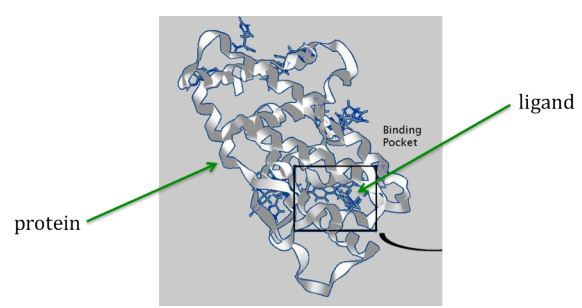
\includegraphics{proteinligand.jpg}
\end{figure}

At a high level, the problem is simple to state: a protein associated with the disease of interest is identified, and its three-dimensional structure is found either experimentally or through a molecular modeling computation. A collection of ligands is tested against the protein: for example, for every orientation of the ligand relative to the protein, computation is done to test whether the ligand binds with the protein in useful ways (such as tying up a biologically active region on the protein). A score is set based on these binding properties, and the best scores are flagged, identifying ligands that would make good drug candidates.


\subsection{Algorithmic Strategy}
\label{intro/intro:algorithmic-strategy}
We will apply a \emph{map-reduce} strategy to this problem, which can be implemented using a \emph{master-worker} design pattern.

Our map-reduce strategy uses three stages of processing.
\begin{enumerate}
\item {} 
First, we will generate many ligands to be tested agains a given protein, using a function \code{Generate\_tasks().} This function produces many \code{{[}ligand, protein{]}} pairs (in this case, all with the same protein) for the next stage.

\item {} 
Next, we will apply a \code{Map()} function to each ligand and the given protein,       which will compute the binding score for that \code{{[}ligand, protein{]}} pair. This \code{Map()} function will produce a pair \code{{[}score, ligand{]}} since we want to know the highest-scoring ligands.

\item {} 
Finally, we identify the ligands with the highest scores, using a function \code{Reduce()} applied to the \code{{[}score, ligand{]}} pairs.

\end{enumerate}

These functions could be implemented sequentially, or they can be called by multiple processes or threads to perform the drug-design computation in parallel: one process, called the \emph{master}, can fill a task queue with pairs obtained from \code{Generate\_tasks().}
Many \emph{worker} processes can pull tasks off the task queue and apply the function \code{Map()} to them. The master can then collect results from the workers and apply \code{Reduce()} to determine the highest-scoring ligand(s).

Note that if the \code{Reduce()} function is expensive to apply, or if the stream of \code{{[}score, ligand{]}} pairs produced by calls to \code{Map()} becomes too large, the \code{Reduce()} stage may be parallelized as well.

This map-reduce approach has been used on clusters and large \href{http://en.wikipedia.org/wiki/Non-Uniform\_Memory\_Access}{NUMA} machines. Stanford University's \href{http://folding.stanford.edu/}{Folding@home} project also involves using idle processing resources from thousands of volunteers' personal computers to run computations on protein folding and related diseases.


\subsection{Simplified Problem Definition}
\label{intro/intro:simplified-problem-definition}
Working with actual ligand and protein data is beyond the scope of this example, so we will represent the computation by a simpler string-based comparison.

Specifically, we simplify the computation as follows:
\begin{quote}
\begin{itemize}
\item {} 
Proteins and ligands will be represented as (randomly-generated) character strings.

\item {} 
The docking-problem computation will be represented by comparing a ligand string \code{L} to a protein string \code{P}.  The score for a pair \code{{[}L, P{]}} will be the maximum number of matching characters among all possibilities when \code{L} is compared to \code{P}, moving from left to right, allowing possible insertions and deletions.  For example, if \code{L} is the string “cxtbcrv” and \code{P} is the string “lcacxtqvivg,” then the score is 4, arising from this comparison of \code{L} to a segment of \code{P}:

\end{itemize}
\begin{figure}[htbp]
\centering

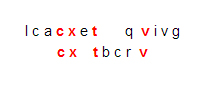
\includegraphics{seq1.jpg}
\end{figure}
\end{quote}

This is not the only comparison of that ligand to that protein that yields four matching characters. Another one is
\begin{quote}
\begin{figure}[htbp]
\centering

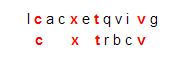
\includegraphics{seq2.jpg}
\end{figure}
\end{quote}

However, there is no comparison that matches five characters while moving from left to right, so the score is 4.


\section{A Sequential Solution}
\label{sequentialimplementation/sequentialimplementation:a-sequential-solution}\label{sequentialimplementation/sequentialimplementation::doc}\label{sequentialimplementation/sequentialimplementation:folding-home}
Let's first examine a traditional sequential (also called serial) solution that uses no parallelism, of the simplified version of this algorithm described in the previous chapter. As with many parallel implementations of algorithms, this serial version can form the basis for a parallel solution. We will later see several parallel solutions that have been updated from the following serial version.

You will want to examine the code itself while reading this chapter.


\subsection{Implementation}
\label{sequentialimplementation/sequentialimplementation:implementation}
In the complete archive, \code{dd.tar.gz}, this example is under the dd/serial directory.

Alternatively, for this chapter, these are the individual files to download:

\code{dd\_serial.cpp}

\code{Makefile}

The Makefile is for use on linux systems.

The example program  provides a sequential C++ implementation of our simplified drug design problem.
\begin{quote}

\begin{notice}{note}{Note:}
The program optionally accepts up to three command-line arguments:
\begin{enumerate}
\item {} 
maximum length of the (randomly generated) ligand strings

\item {} 
number of ligands generated

\item {} 
protein string to which ligands will be compared

\end{enumerate}
\end{notice}
\end{quote}


\subsection{Compilation:}
\label{sequentialimplementation/sequentialimplementation:compilation}
A straightforward compile can be used for this sequential example:
\begin{quote}

g++ -o dd\_serial dd\_serial.cpp
\end{quote}

Or you can use the makefile and simply type `make' at the command line on a linux system.


\subsubsection{The Code}
\label{sequentialimplementation/sequentialimplementation:the-code}
In this implementation, the class \code{MR} encapsulates the map-reduce steps \code{Generate\_tasks()}, \code{Map()}, and \code{Reduce()} as private methods (member functions of the class), and a public method \code{run()} invokes those steps according to a map-reduce algorithmic strategy (see previous Introduction section for detailed explanation). We have highlighted calls to the methods representing map-reduce steps in the following code segment from \code{MR::run()}.
\begin{quote}

\begin{Verbatim}[commandchars=\\\{\}]
\PYG{n}{Generate\PYGZus{}tasks}\PYG{p}{(}\PYG{n}{tasks}\PYG{p}{)}\PYG{p}{;}
\PYG{c+c1}{// assert -- tasks is non-empty}

\PYG{k}{while} \PYG{p}{(}\PYG{o}{!}\PYG{n}{tasks}\PYG{p}{.}\PYG{n}{empty}\PYG{p}{(}\PYG{p}{)}\PYG{p}{)} \PYG{p}{\PYGZob{}}
  \PYG{n}{Map}\PYG{p}{(}\PYG{n}{tasks}\PYG{p}{.}\PYG{n}{front}\PYG{p}{(}\PYG{p}{)}\PYG{p}{,} \PYG{n}{pairs}\PYG{p}{)}\PYG{p}{;}
  \PYG{n}{tasks}\PYG{p}{.}\PYG{n}{pop}\PYG{p}{(}\PYG{p}{)}\PYG{p}{;}
\PYG{p}{\PYGZcb{}}

\PYG{n}{do\PYGZus{}sort}\PYG{p}{(}\PYG{n}{pairs}\PYG{p}{)}\PYG{p}{;}

\PYG{k+kt}{int} \PYG{n}{next} \PYG{o}{=} \PYG{l+m+mi}{0}\PYG{p}{;}  \PYG{c+c1}{// index of first unprocessed pair in pairs[]}
\PYG{k}{while} \PYG{p}{(}\PYG{n}{next} \PYG{o}{\PYGZlt{}} \PYG{n}{pairs}\PYG{p}{.}\PYG{n}{size}\PYG{p}{(}\PYG{p}{)}\PYG{p}{)} \PYG{p}{\PYGZob{}}
  \PYG{n}{string} \PYG{n}{values}\PYG{p}{;}
  \PYG{n}{values} \PYG{o}{=} \PYG{l+s}{"}\PYG{l+s}{"}\PYG{p}{;}
  \PYG{k+kt}{int} \PYG{n}{key} \PYG{o}{=} \PYG{n}{pairs}\PYG{p}{[}\PYG{n}{next}\PYG{p}{]}\PYG{p}{.}\PYG{n}{key}\PYG{p}{;}
  \PYG{n}{next} \PYG{o}{=} \PYG{n}{Reduce}\PYG{p}{(}\PYG{n}{key}\PYG{p}{,} \PYG{n}{pairs}\PYG{p}{,} \PYG{n}{next}\PYG{p}{,} \PYG{n}{values}\PYG{p}{)}\PYG{p}{;}
  \PYG{n}{Pair} \PYG{n}{p}\PYG{p}{(}\PYG{n}{key}\PYG{p}{,} \PYG{n}{values}\PYG{p}{)}\PYG{p}{;}
  \PYG{n}{results}\PYG{p}{.}\PYG{n}{push\PYGZus{}back}\PYG{p}{(}\PYG{n}{p}\PYG{p}{)}\PYG{p}{;}
\PYG{p}{\PYGZcb{}}
\end{Verbatim}
\end{quote}


\subsubsection{Comments}
\label{sequentialimplementation/sequentialimplementation:comments}\begin{itemize}
\item {} 
We use the \href{http://www.cplusplus.com/reference/stl/}{STL containers}  \code{queue\textless{}\textgreater{}}  and  \code{vector\textless{}\textgreater{}}  to hold the results from each of the map-reduce steps: namely, the task queue of ligands to process, the list key-value pairs produced by the \code{Map()} phase, and the list of resulting key-value pairs produced by calls to \code{Reduce()}. We define those container variables as data members in the class \code{MR}:
\begin{quote}

\code{queue\textless{}string\textgreater{} tasks;}

\code{vector\textless{}Pair\textgreater{} pairs, results;}
\end{quote}

\item {} 
Here, \code{Pair} is a struct representing key-value pairs with the desired types:

\begin{Verbatim}[commandchars=\\\{\}]
\PYG{k}{struct} \PYG{n}{Pair} \PYG{p}{\PYGZob{}}
  \PYG{k+kt}{int} \PYG{n}{key}\PYG{p}{;}
  \PYG{n}{string} \PYG{n}{val}\PYG{p}{;}
  \PYG{n}{Pair}\PYG{p}{(}\PYG{k+kt}{int} \PYG{n}{k}\PYG{p}{,} \PYG{k}{const} \PYG{n}{string} \PYG{o}{\PYGZam{}}\PYG{n}{v}\PYG{p}{)} \PYG{p}{\PYGZob{}}\PYG{n}{key}\PYG{o}{=}\PYG{n}{k}\PYG{p}{;} \PYG{n}{val}\PYG{o}{=}\PYG{n}{v}\PYG{p}{;}\PYG{p}{\PYGZcb{}}
\PYG{p}{\PYGZcb{}}\PYG{p}{;}
\end{Verbatim}

\item {} 
In the example code, \code{Generate\_tasks()} merely produces \emph{nligands} strings of random lower-case letters, each having a random length between 0 and \emph{max\_ligand}. The program stores those strings in a task queue named \code{tasks}.

\item {} 
For each ligand in the task queue, the \code{Map()} function computes the match score from comparing a string representing that ligand to a global string representing a target protein, using the simplified match-scoring algorithm described above. \code{Map()} then yields a key-value pair consisting of that score and that ligand, respectively.

\item {} 
The key-value pairs produced by all calls to \code{Map()} are sorted by key in order to group pairs with the same score. Then \code{Reduce()} is called once for each of those groups in order to yield a vector of \code{Pairs} consisting of a score \emph{s} together with a list of all ligands whose best score was \emph{s}.

\begin{notice}{note}{Note:}
Map-reduce frameworks such as the open-source Hadoop commonly use sorting to group values for a given key, as does our program. This has the additional benefit of producing sorted results from the reduce stage. Also, the staged processes of performing all \code{Map()} calls before sorting and of performing all \code{Reduce()} calls after the completion of sorting are also common among map-reduce frameworks.
\end{notice}

\item {} 
The methods \code{Generate\_tasks()}, \code{Map()}, and \code{Reduce()} may seem like unnecessary complication for this problem since they abstract so little code. Indeed, we could certainly rewrite the program more simply and briefly without them. We chose this expression for several reasons:
\begin{itemize}
\item {} 
We can compare code segments from \code{MR::run()} directly with corresponding segments in upcoming parallel implementations to focus on the parallelization changes and hide the common code in method calls.

\item {} 
The methods \code{Generate\_tasks()}, \code{Map()}, and \code{Reduce()} make it obvious where to insert more realistic task generation, docking algorithm, etc., and where to change our map-reduce code examples for problems other than drug design.

\item {} 
We use these three method names in descriptions of the map-reduce pattern elsewhere.

\end{itemize}

\item {} 
We have not attempted to implement the fault tolerance and scalability features of a production map-reduce framework such as Hadoop.

\end{itemize}


\subsubsection{Questions for Exploration}
\label{sequentialimplementation/sequentialimplementation:questions-for-exploration}\label{sequentialimplementation/sequentialimplementation:stl-containers}\begin{itemize}
\item {} 
Compile and test run the sequential program. Determine values for the command-line arguments \code{max\_ligand{}`{}`(maximum length of a ligand string) and {}`{}`nligands} (total number of ligands to process) that lead to a tolerably long computation for experimenting (e.g., perhaps 15 seconds to a minute of computation). Note the following about our simplified computational problem:
\begin{itemize}
\item {} 
Our stand-in scoring algorithm is exponential in the lengths of the ligand and protein strings. Thus, a large value of \code{max\_ligand} may cause an extremely lengthy computation. Altering \code{max\_ligand} can help in finding a test computation of a desired order of magnitude.

\item {} 
We expect the computation time to increase approximately linearly with the number of ligands \code{nligands}. However, if \code{nligands} is relatively small, you may notice irregular jumps to long computation times when increasing \code{nligands}. This is because our simple random algorithm for generating ligands produces ligand strings using \code{random()}, as well as ligands with random lengths as well as random content.  Because of the order-of-magnitude effect of ligand length, a sudden long ligand (meaning more characters than those before) may greatly increase the computation time.

\end{itemize}

\item {} 
If you have \emph{more realistic algorithms for docking and/or more realistic data for ligands and proteins}, modify the program to incorporate those elements, and compare the results from your modified program to results obtained by other means (other software, wet-lab results, etc.).

\end{itemize}


\section{OpenMP Solution}
\label{openmp/openmp:openmp-solution}\label{openmp/openmp::doc}
In the complete archive, \code{dd.tar.gz}, this example is under the dd/openMP directory.

Alternatively, for this chapter, these are the individual files to download:

\code{dd\_omp.cpp}

\code{Makefile}

The Makefile is for use on linux systems.

Here, we implement our drug design simulation in parallel using OpenMP, an API that provides compiler directives, library routines, and environment variables that allow shared-memory multithreading in C/C++. A master thread will fork off a specified number of worker threads and assign parts of a task to them (read \href{http://en.wikipedia.org/wiki/OpenMP}{more}).


\subsection{Implementation}
\label{openmp/openmp:implementation}
The implementation dd\_omp.cpp parallelizes the \code{Map()} loop using OpenMP and uses a thread-safe container from \href{http://en.wikipedia.org/wiki/Intel\_Threading\_Building\_Blocks}{TBB}, a C++ template library designed to help avoid some of the difficulties associated with multithreading.

Since we expect the docking algorithm (here represented by computing a match score for comparing a ligand string to a protein string) to require the bulk of compute time, we will parallelize the \code{Map()} stage in our sequential algorithm. The loop to be parallelized is shown below, from the full sequential implementation, dd\_serial.cpp, discussed in the previous chapter.

\begin{Verbatim}[commandchars=\\\{\}]
\PYG{k}{while} \PYG{p}{(}\PYG{o}{!}\PYG{n}{tasks}\PYG{p}{.}\PYG{n}{empty}\PYG{p}{(}\PYG{p}{)}\PYG{p}{)} \PYG{p}{\PYGZob{}}
        \PYG{n}{Map}\PYG{p}{(}\PYG{n}{tasks}\PYG{p}{.}\PYG{n}{front}\PYG{p}{(}\PYG{p}{)}\PYG{p}{,} \PYG{n}{pairs}\PYG{p}{)}\PYG{p}{;}
        \PYG{n}{tasks}\PYG{p}{.}\PYG{n}{pop}\PYG{p}{(}\PYG{p}{)}\PYG{p}{;}
\PYG{p}{\PYGZcb{}}
\end{Verbatim}

We will now parallelize this mapping loop by converting it to a \code{for} loop, then applying OpenMP’s \code{parallel for} feature - there is no \code{parallel while}. For easier use with a \code{for} loop, we will replace the \code{tasks} queue with a vector (of the same name) and iterate on index values for that vector.

This causes a potential concurrency problem, though, because multiple OpenMP threads will now each be calling \code{Map()}, and those multiple calls by parallel threads may overlap. There is no potential for error from the first argument \code{ligand} of \code{Map()}, since \code{Map()} requires simply read-only access for that argument. However, multiple calls of \code{Map()} in different threads might interfere with each other when changing the writable second argument \code{pairs} of \code{Map()}, leading to a data race condition. The STL containers are \emph{not} thread safe, meaning that they provide no protection against such interference, and errors may result.

Therefore, we will use TBB’s thread-safe \code{concurrent\_vector} container for \code{pairs}, leading to the following code segments in our OpenMP implementation.

\begin{Verbatim}[commandchars=\\\{\}]
\PYG{n}{vector}\PYG{o}{\PYGZlt{}}\PYG{n}{string}\PYG{o}{\PYGZgt{}} \PYG{n}{tasks}\PYG{p}{;}
\PYG{n}{tbb}\PYG{o}{:}\PYG{o}{:}\PYG{n}{concurrent\PYGZus{}vector}\PYG{o}{\PYGZlt{}}\PYG{n}{Pair}\PYG{o}{\PYGZgt{}} \PYG{n}{pairs}\PYG{p}{;}
\PYG{n}{vector}\PYG{o}{\PYGZlt{}}\PYG{n}{Pair}\PYG{o}{\PYGZgt{}} \PYG{n}{results}\PYG{p}{;}

\PYG{n}{Generate\PYGZus{}tasks}\PYG{p}{(}\PYG{n}{tasks}\PYG{p}{)}\PYG{p}{;}
\PYG{c+c1}{// assert -- tasks is non-empty}

\PYG{c+cp}{\PYGZsh{}}\PYG{c+cp}{pragma omp parallel for num\PYGZus{}threads(nthreads)}
        \PYG{k}{for} \PYG{p}{(}\PYG{k+kt}{int} \PYG{n}{t} \PYG{o}{=} \PYG{l+m+mi}{0}\PYG{p}{;}  \PYG{n}{t} \PYG{o}{\PYGZlt{}} \PYG{n}{tasks}\PYG{p}{.}\PYG{n}{size}\PYG{p}{(}\PYG{p}{)}\PYG{p}{;}  \PYG{n}{t}\PYG{o}{+}\PYG{o}{+}\PYG{p}{)} \PYG{p}{\PYGZob{}}
                \PYG{n}{Map}\PYG{p}{(}\PYG{n}{tasks}\PYG{p}{[}\PYG{n}{t}\PYG{p}{]}\PYG{p}{,} \PYG{n}{pairs}\PYG{p}{)}\PYG{p}{;}
        \PYG{p}{\PYGZcb{}}
\end{Verbatim}

Since the main thread (i.e., the thread that executes \code{run()}) is the only thread that performs the stages that call \code{Generate\_tasks()}, \code{to\_sort()}, and \code{Reduce()}, it is safe for the vectors \code{tasks} or \code{results} to remain implemented as (non-thread safe) STL containers.  See the implementation (dd\_omp.cpp) for complete details.


\subsection{Further Notes}
\label{openmp/openmp:further-notes}\label{openmp/openmp:tbb}\begin{itemize}
\item {} 
Most of the changes between the sequential version and this OpenMP version arise from the change in type for the data member \code{MR::pairs} to a \emph{thread-safe} data type; a few changes have to do with managing the number of threads to use \code{nthreads}. All of the \emph{parallel} computation is specified by the one-line \code{\#pragma} directive shown above - without it, the computation would proceed sequentially.

\item {} 
This OpenMP implementation has four (optional) command-line arguments.  The third argument specifies the number of OpenMP threads to use (note that this differs from the third argument in the sequential version). In dd\_omp.cpp, the command-line arguments have these effects:
\begin{enumerate}
\item {} 
maximum length of a (randomly generated) ligand string

\item {} 
number of ligands generated

\item {} 
number of OpenMP threads to request

\item {} 
protein string to which ligands will be compared

\end{enumerate}

\end{itemize}


\subsection{Questions for Exploration}
\label{openmp/openmp:questions-for-exploration}\begin{itemize}
\item {} 
Compare the performance of dd\_serial.cpp with dd\_omp.cpp on a multicore computer using the same values for \code{max\_ligand} and \code{nligands}. Do you observe speedup for the parallel version?

\item {} 
Our development system has four cores, and \code{nthreads=4} was used for one of our test runs. We found that the omp version performed about \emph{three} times as fast as :the serial version for the same values of \code{max\_ligand} and \code{nligands}. Can you explain why it didn’t perform four times as fast?

\item {} 
Use the command-line arguments to experiment with varying the number of OpenMP threads in an invocation of dd\_omp.cpp, while holding \code{max\_ligand} and \code{nligands} unchanged. On a multi-core system, we hope for better performance when more threads are used. Do you observe such performance improvement when you time the execution? What happens when the number of threads exceeds the number of cores (or hyperthreads) on your system? Explain as much as you can about the timing results you observe when you vary the number of threads.

\item {} 
You may notice that dd\_omp.cpp computes the same maximal score and identifies the same ligands as the serial version that produces that score, but if more than one ligand yields the maximal score, the \emph{order} of those maximal-scoring ligands may differ between the two versions. Can you explain why?

\item {} 
Our sequential program always produces the same results for given values of the \code{max\_ligand}, \code{nligands},  and \code{protein} command-line arguments. This is because we use the default random-number seed in our code. Because of this consistency, we can describe the sequential version as being a \emph{deterministic} computation. Is dd\_omp.cpp a deterministic computation? Explain your answer, and/or state what more you need to know in order to answer this question.

\item {} 
If you have \emph{more realistic algorithms for docking and/or more realistic data for ligands and proteins}, modify the openMP program to incorporate those elements, and compare the results from your modified program to results obtained by other means (other software, wet-lab results, etc.). How does the performance of your modified OpenMP version compare to what you observed from your modified sequential version?

\item {} 
Whereas our serial implementation used a queue data structure for \code{tasks}, this implementation uses a vector data structure, and parallelizes the “map” stage using OpenMP’s \code{omp parallel for} pragma. This suffices for our simplified example, because we generate all ligands before processing any of them. However, some computations require a task queue, since processing some tasks may generate others (not out of the question for drug design, since high-scoring ligands might lead one to consider similar ligands in search of even higher scores). \textbf{Challenge problem:} Modify dd\_omp.cpp to use a task \emph{queue} instead of a task vector.
\begin{quote}

\begin{notice}{note}{Note:}\begin{itemize}
\item {} 
Use a thread-safe queue data structure for \code{tasks}, such as \code{tbb::concurrent\_queue} or \code{tbb::concurrent\_bounded\_queue}, because multiple threads may attempt to modify the queue at the same time.

\item {} 
Instead of \code{omp parallel for}, use OpenMP 3.0 tasks.  You can parallelize a \code{while} loop that moves through the task queue using \code{omp parallel} to enclose that loop.

\item {} 
Depending on your algorithm, it may help to use “sentinel” values, as described in Chapter 8 of \href{http://books.google.com/books/about/The\_Art\_of\_Concurrency.html?id=rU68SYVS7S8C}{this book} or as used by the Boost threads implementation in the next page.

\end{itemize}
\end{notice}
\end{quote}

\end{itemize}


\section{C++11 Threads Solution}
\label{c++11threads/c++11threads:c-11-threads-solution}\label{c++11threads/c++11threads:this-book}\label{c++11threads/c++11threads::doc}
In the complete archive, \code{dd.tar.gz}, this example is under the dd/threads directory.

Alternatively, for this chapter, these are the individual files to download:

\code{dd\_threads.cpp}

\code{Makefile}

The Makefile is for use on linux systems.

In the OpenMP implementation, the OpenMP runtime system implicitly creates and manages threads for us. The dd\_threads.cpp implementation parallelizes the computationally expensive \code{Map()} stage by using the new C++11 standard threads instead of OpenMP. This requires us to explicitly create and manage our own threads, using a master-worker parallel programming pattern driven by \code{tasks}, and a task queue produced by \code{Generate\_tasks()}.

We will examine the C++11 threads implementation  by comparing it to the sequential implementation. You may want to have each of them open in an editor as you read along.

The main routine for map-reduce computing in both implementations is \code{MR::run()}, and this routine is identical in the two except for the “map” stage and for the threads version handling an extra argument \code{nthreads}. In the serial implementation, the “map” stage simply removes elements from the task queue and calls \code{Map()} for each such element, via the following code.
\begin{quote}

\begin{Verbatim}[commandchars=\\\{\}]
\PYG{k}{while} \PYG{p}{(}\PYG{o}{!}\PYG{n}{tasks}\PYG{p}{.}\PYG{n}{empty}\PYG{p}{(}\PYG{p}{)}\PYG{p}{)} \PYG{p}{\PYGZob{}}
        \PYG{n}{Map}\PYG{p}{(}\PYG{n}{tasks}\PYG{p}{.}\PYG{n}{front}\PYG{p}{(}\PYG{p}{)}\PYG{p}{,} \PYG{n}{pairs}\PYG{p}{)}\PYG{p}{;}
        \PYG{n}{tasks}\PYG{p}{.}\PYG{n}{pop}\PYG{p}{(}\PYG{p}{)}\PYG{p}{;}
\PYG{p}{\PYGZcb{}}
\end{Verbatim}
\end{quote}

However, the threads implementation of the “map” stage creates an array \code{pool} of threads to perform the calls to \code{Map()}, then waits for those threads to complete their work by calling the \code{join()} method for each thread:
\begin{quote}

\begin{Verbatim}[commandchars=\\\{\}]
\PYG{k+kr}{thread} \PYG{o}{*}\PYG{n}{pool} \PYG{o}{=} \PYG{k}{new} \PYG{k+kr}{thread}\PYG{p}{[}\PYG{n}{nthreads}\PYG{p}{]}\PYG{p}{;}
\PYG{k}{for} \PYG{p}{(}\PYG{k+kt}{int} \PYG{n}{i} \PYG{o}{=} \PYG{l+m+mi}{0}\PYG{p}{;}  \PYG{n}{i} \PYG{o}{\PYGZlt{}} \PYG{n}{nthreads}\PYG{p}{;}  \PYG{n}{i}\PYG{o}{+}\PYG{o}{+}\PYG{p}{)}
\PYG{n}{pool}\PYG{p}{[}\PYG{n}{i}\PYG{p}{]} \PYG{o}{=} \PYG{k+kr}{thread}\PYG{p}{(}\PYG{o}{\PYGZam{}}\PYG{n}{MR}\PYG{o}{:}\PYG{o}{:}\PYG{n}{do\PYGZus{}Maps}\PYG{p}{,} \PYG{k}{this}\PYG{p}{)}\PYG{p}{;}


\PYG{k}{for} \PYG{p}{(}\PYG{k+kt}{int} \PYG{n}{i} \PYG{o}{=} \PYG{l+m+mi}{0}\PYG{p}{;}  \PYG{n}{i} \PYG{o}{\PYGZlt{}} \PYG{n}{nthreads}\PYG{p}{;}  \PYG{n}{i}\PYG{o}{+}\PYG{o}{+}\PYG{p}{)}
\PYG{n}{pool}\PYG{p}{[}\PYG{n}{i}\PYG{p}{]}\PYG{p}{.}\PYG{n}{join}\PYG{p}{(}\PYG{p}{)}\PYG{p}{;}
\end{Verbatim}
\end{quote}

In this snippet from the threads implementation, we define the function \code{MR::do\_Maps()} for performing calls to \code{Map()}:
\begin{quote}

\begin{Verbatim}[commandchars=\\\{\}]
\PYG{k+kt}{void} \PYG{n}{MR}\PYG{o}{:}\PYG{o}{:}\PYG{n}{do\PYGZus{}Maps}\PYG{p}{(}\PYG{k+kt}{void}\PYG{p}{)} \PYG{p}{\PYGZob{}}
        \PYG{n}{string} \PYG{n}{lig}\PYG{p}{;}
        \PYG{n}{tasks}\PYG{p}{.}\PYG{n}{pop}\PYG{p}{(}\PYG{n}{lig}\PYG{p}{)}\PYG{p}{;}
        \PYG{k}{while} \PYG{p}{(}\PYG{n}{lig} \PYG{o}{!}\PYG{o}{=} \PYG{n}{SENTINEL}\PYG{p}{)} \PYG{p}{\PYGZob{}}
                \PYG{n}{Map}\PYG{p}{(}\PYG{n}{lig}\PYG{p}{,} \PYG{n}{pairs}\PYG{p}{)}\PYG{p}{;}
                \PYG{n}{tasks}\PYG{p}{.}\PYG{n}{pop}\PYG{p}{(}\PYG{n}{lig}\PYG{p}{)}\PYG{p}{;}
        \PYG{p}{\PYGZcb{}}
        \PYG{n}{tasks}\PYG{p}{.}\PYG{n}{push}\PYG{p}{(}\PYG{n}{SENTINEL}\PYG{p}{)}\PYG{p}{;}  \PYG{c+c1}{// restore end marker for another thread}
\PYG{p}{\PYGZcb{}}
\end{Verbatim}
\end{quote}

This method \code{do\_Maps()} serves as the “main program” for each thread, and that method repeatedly pops a new ligand string \code{lig} from the task queue, and calls \code{Map()} with \code{lig} until it encounters the end marker \code{SENTINEL}.

Since multiple threads may access the shared task queue \code{tasks} at the same time, that task queue must be thread-safe, so we defined it using a TBB container:
\begin{quote}

\code{tbb::concurrent\_bounded\_queue\textless{}string\textgreater{} tasks;}
\end{quote}

We chose \code{tbb::concurrent\_bounded\_queue} instead of \code{tbb::concurrent\_queue} because the bounded type offers a blocking \code{pop()} method, which will cause a thread to wait until work becomes available in the queue; also, we do not anticipate a need for a task queue of unbounded size. Blocking on the task queue isn’t actually necessary for our simplified application, because all the tasks are generated before any of the threads begin operating on those tasks. However, this blocking strategy supports a \emph{dynamic} task queue, in which new tasks can be added to the queue while other tasks are being processed, a requirement that often arises in other applications.


\subsection{Further Notes}
\label{c++11threads/c++11threads:further-notes}\begin{itemize}
\item {} 
The \code{SENTINEL} task value indicates that no more tasks remain. Each thread consumes one \code{SENTINEL} from the task queue so it can know when to exit, and adds one \code{SENTINEL} to the task queue just before that thread exits, which then enables another thread to finish.

\item {} 
As with the OpenMP version, the  threads implementation uses a thread-safe vector (\code{tbb::concurrent\_vector\textless{}Pair\textgreater{} pairs;}) for storing the key-value pairs produced by calls to \code{Map()}, since multiple threads might access that shared vector at the same time.

\end{itemize}


\subsection{Questions for exploration}
\label{c++11threads/c++11threads:questions-for-exploration}\begin{itemize}
\item {} 
Compile and run the code, and compare its performance to the serial version and to other parallel implementations.

\item {} 
\emph{Concurrent task queue:} consider the “map” stage in our sequential implementation, which uses an STL container instead of a TBB container for the task queue \code{tasks}:
\begin{quote}

\begin{Verbatim}[commandchars=\\\{\}]
\PYG{k}{while} \PYG{p}{(}\PYG{o}{!}\PYG{n}{tasks}\PYG{p}{.}\PYG{n}{empty}\PYG{p}{(}\PYG{p}{)}\PYG{p}{)} \PYG{p}{\PYGZob{}}
        \PYG{n}{Map}\PYG{p}{(}\PYG{n}{tasks}\PYG{p}{.}\PYG{n}{front}\PYG{p}{(}\PYG{p}{)}\PYG{p}{,} \PYG{n}{pairs}\PYG{p}{)}\PYG{p}{;}
        \PYG{n}{tasks}\PYG{p}{.}\PYG{n}{pop}\PYG{p}{(}\PYG{p}{)}\PYG{p}{;}
\PYG{p}{\PYGZcb{}}
\end{Verbatim}

\begin{notice}{note}{Note:}\begin{itemize}
\item {} 
TBB container classes \code{tbb::concurrent\_queue} and \code{tbb::concurrent\_bounded\_queue} do not provide a method \code{front()}. Instead, they provide a method \code{try\_pop()} (with one argument). It works as follows: if the queue is empty, it returns immediately (non-blocking) without making any changes. If the queue is non-empty, it removes the first element from the queue and assigns it to the argument. This accomplishes the work of an STL \code{queue}’s \code{front()} and \code{pop()} methods in a single operation. Describe a parallel computing scenario in which a single (atomic) operation \code{try\_pop()} is preferable to separate operations \code{front()} and \code{pop()}, and explain why we should prefer it.

\item {} 
Given that we choose a TBB queue container for the type of \code{tasks}, would it be safe to have multiple threads execute the following code (which more closely mirrors our sequential operation)?
\begin{quote}

\begin{Verbatim}[commandchars=\\\{\}]
\PYG{n}{string} \PYG{n}{lig}\PYG{p}{;}
\PYG{k}{while} \PYG{p}{(}\PYG{o}{!}\PYG{n}{tasks}\PYG{p}{.}\PYG{n}{empty}\PYG{p}{(}\PYG{p}{)}\PYG{p}{)} \PYG{p}{\PYGZob{}}
        \PYG{n}{tasks}\PYG{p}{.}\PYG{n}{try\PYGZus{}pop}\PYG{p}{(}\PYG{n}{lig}\PYG{p}{)}\PYG{p}{;}
        \PYG{n}{Map}\PYG{p}{(}\PYG{n}{lig}\PYG{p}{,} \PYG{n}{pairs}\PYG{p}{)}\PYG{p}{;}
\PYG{p}{\PYGZcb{}}
\end{Verbatim}
\end{quote}

\end{itemize}

If it \emph{is} safe, explain how you know it is so.  If something can go wrong with this code, describe a scenario in which it fails to behave correctly.
\end{notice}
\end{quote}

\item {} 
The purpose of \code{SENTINEL} in our threads implementation is to insure that every (non-\code{SENTINEL}) element in the task queue \code{tasks} is processed by some thread, and that all threads terminate (return from \code{do\_Maps()}) when no more (non-\code{SENTINEL}) elements are available. Verify that this goal is achieved in \code{dd\_threads.cpp}, or describe a scenario in which the goal fails.

\item {} 
Revise dd\_threads.cpp\textgreater{} to use a \code{tbb::concurrent\_queue} container instead of a \code{tbb::concurrent\_bounded\_queue} container for the task queue \code{tasks}.
\begin{quote}

\begin{notice}{note}{Note:}\begin{itemize}
\item {} 
\code{tbb::concurrent\_queue} does not provide the blocking method \code{pop()} used in \code{dd\_threads.cpp}, so some other synchronization strategy will be required.

\item {} 
However, in our simplified problem, the task queue \code{tasks} doesn’t change during the “map” stage, so threads may finish once \code{tasks} becomes empty.

\item {} 
Be sure to understand the concurrent task queue exercise above (italicized) before attempting this exercise.

\item {} 
Is a \code{SENTINEL} value needed for your solution?

\end{itemize}
\end{notice}
\end{quote}

\item {} 
For further ideas, see exercises for other parallel implementations.

\end{itemize}


\section{A Message Passing Interface (MPI) Solution}
\label{mpi/mpi:a-message-passing-interface-mpi-solution}\label{mpi/mpi::doc}
In the complete archive, \code{dd.tar.gz}, this example is under the dd/MPI directory.

Alternatively, for this chapter, these are the individual files to download:

\code{dd\_mpi.cpp}

\code{Makefile}

The Makefile is for use on linux systems.


\subsection{A cluster system}
\label{mpi/mpi:a-cluster-system}
Now we turn to a solution for use on clusters of computer systems. Because each computer in the cluster is a standalone machine, the work will need to be coordinated by distributing it across the machines in separate processes and ccommunicating between those processes using message passing, which is provided by the MPI library.


\subsection{Single Program, Multiple Data}
\label{mpi/mpi:single-program-multiple-data}
This program uses the master-worker strategy within a single program. This strategy is implemented within the \code{run} method of the \code{MR} class. One process, called the root, or master, has the responsibility for:
\begin{itemize}
\item {} 
generating all of the ligand scoring tasks

\item {} 
sending the next available ligand scoring task to a worker when asked

\item {} 
cordinating when all scoring tasks have been completed

\end{itemize}

All of the other processes, called workers, will be responsible for:
\begin{itemize}
\item {} 
asking the master for some work by sending that process a message

\item {} 
receiving the work and computing the score for that ligand

\end{itemize}

In the code, the separation of these tasks is done by keeping track of the \emph{rank} of each process (a unique number given to each process that was initialized) and using it to determine what it will do. In this code, this line indicates the section of code for the master (by tradition number 0):
\begin{quote}

\begin{Verbatim}[commandchars=\\\{\}]
\PYG{k}{if} \PYG{p}{(}\PYG{n}{rank} \PYG{o}{=}\PYG{o}{=} \PYG{n}{root}\PYG{p}{)} \PYG{p}{\PYGZob{}}
\end{Verbatim}
\end{quote}

and the else block corresponding to this if statement holds the code that each worker process on other machines will execute. This way of indicating code for different types of processes (master and worker) within the same program is commonly refered to as the single-program, multiple data software pattern in parallel and distributed computing. The MPI library was designed to use this pattern in this manner.

In a cluster, memory is not shared between all processes, so not every worker process running on a different machine will have a copy of the vector containing the pairs of processed ligands and their scores. This will be maintained by the master, or root process. Because of this, the Map function found in previous examples that looked like this:
\begin{quote}

\begin{Verbatim}[commandchars=\\\{\}]
\PYG{k+kt}{void} \PYG{n}{MR}\PYG{o}{:}\PYG{o}{:}\PYG{n}{Map}\PYG{p}{(}\PYG{k}{const} \PYG{n}{string} \PYG{o}{\PYGZam{}}\PYG{n}{ligand}\PYG{p}{,} \PYG{n}{tbb}\PYG{o}{:}\PYG{o}{:}\PYG{n}{concurrent\PYGZus{}vector}\PYG{o}{\PYGZlt{}}\PYG{n}{Pair}\PYG{o}{\PYGZgt{}} \PYG{o}{\PYGZam{}}\PYG{n}{pairs}\PYG{p}{)} \PYG{p}{\PYGZob{}}
  \PYG{n}{Pair} \PYG{n}{p}\PYG{p}{(}\PYG{n}{Help}\PYG{o}{:}\PYG{o}{:}\PYG{n}{score}\PYG{p}{(}\PYG{n}{ligand}\PYG{p}{.}\PYG{n}{c\PYGZus{}str}\PYG{p}{(}\PYG{p}{)}\PYG{p}{,} \PYG{n}{protein}\PYG{p}{.}\PYG{n}{c\PYGZus{}str}\PYG{p}{(}\PYG{p}{)}\PYG{p}{)}\PYG{p}{,} \PYG{n}{ligand}\PYG{p}{)}\PYG{p}{;}
  \PYG{n}{pairs}\PYG{p}{.}\PYG{n}{push\PYGZus{}back}\PYG{p}{(}\PYG{n}{p}\PYG{p}{)}\PYG{p}{;}
\PYG{p}{\PYGZcb{}}
\end{Verbatim}
\end{quote}

now must be split up between the workers, who will do the scoring, and the master, who will take on the task of pushing the result received from each worker back onto the vector. Take note of where the score method is called in the worker portion of the \code{run} function of the MR class, and the result is sent to the master process. Then note where that score is received in the master process section of the code and pushed onto the pairs vector.


\subsection{Questions for Explortion}
\label{mpi/mpi:questions-for-explortion}\begin{itemize}
\item {} 
Compile and run the code on a cluster (using mpirun). Generally speaking, does it seem faster for a given set of problem sizes (number of ligands, size of input protein string). As you add processes, does it seem to get faster?

\item {} 
Investigate how to time how long the code takes to run, using a function called \emph{MPI\_get\_wtime()}. Improve this code by adding the capability to determine its running time and report it with the results.

\item {} 
What issues arise with timing code like this when the ligands are randomly generated?

\end{itemize}


\section{Go Solution}
\label{go/go::doc}\label{go/go:go-solution}
In the complete archive, \code{dd.tar.gz}, this example is under the dd/go directory.

Alternatively, for this chapter, this is the individual file to download:

\code{dd\_go.go}

You will also need to refer to the C++11 threads solution, found in the dd/threads directory in the full archive or available individually:

\code{dd\_threads.cpp}

Google’s Go language makes it possible to program with implicitly launched threads, and its channel feature enables simplified thread-safe processing of shared data.

We will compare the “map” stage in the Go implementation to the “map” stage in the C++11 thread code. The segment of \code{main()} in dd\_go.go that implements the “map” stage appears below.
\begin{quote}

\begin{Verbatim}[commandchars=\\\{\}]
\PYG{n}{pairs} \PYG{p}{:=} \PYG{n+nb}{make}\PYG{p}{(}\PYG{k}{chan} \PYG{n}{Pair}\PYG{p}{,} \PYG{l+m+mi}{1024}\PYG{p}{)}
\PYG{k}{for} \PYG{n}{i} \PYG{p}{:=} \PYG{l+m+mi}{0}\PYG{p}{;} \PYG{n}{i} \PYG{p}{\PYGZlt{}} \PYG{p}{*}\PYG{n}{nCPU}\PYG{p}{;} \PYG{n}{i}\PYG{p}{++} \PYG{p}{\PYGZob{}}
\PYG{k}{go} \PYG{k}{func}\PYG{p}{(}\PYG{p}{)} \PYG{p}{\PYGZob{}}
                \PYG{n}{p} \PYG{p}{:=} \PYG{p}{[}\PYG{p}{]}\PYG{n+nb}{byte}\PYG{p}{(}\PYG{p}{*}\PYG{n}{protein}\PYG{p}{)}
                \PYG{k}{for} \PYG{n}{l} \PYG{p}{:=} \PYG{k}{range} \PYG{n}{ligands} \PYG{p}{\PYGZob{}}
                        \PYG{n}{pairs} \PYG{p}{\PYGZlt{}-} \PYG{n}{Pair}\PYG{p}{\PYGZob{}}\PYG{n}{score}\PYG{p}{(}\PYG{n}{l}\PYG{p}{,} \PYG{n}{p}\PYG{p}{)}\PYG{p}{,} \PYG{n}{l}\PYG{p}{\PYGZcb{}}
                \PYG{p}{\PYGZcb{}}
        \PYG{p}{\PYGZcb{}}\PYG{p}{(}\PYG{p}{)}
\PYG{p}{\PYGZcb{}}
\end{Verbatim}
\end{quote}

Instead of a vector of \code{Pair} as in dd\_threads.cpp, the Go implementation creates a \emph{channel} object called \code{pairs} for communicating \code{Pair} objects through message passing. The “map” stage will send \code{Pair}s into the channel \code{pairs}, and the sorting stage will receive those \code{Pair}s from that same channel. In effect, channel \code{pairs} behaves like a queue, in which the send operation (\code{\textless{}-}) functions like \code{push\_back} and the receive operation (also \code{\textless{}-}, but with the channel on the right side; not shown in the snippet above) acts like \code{pop}.

The C++11 threads implementation allocated an array \code{pool} of threads, then had each thread call \code{do\_Map()} in order to carry out that thread’s work in the “map” stage. The following code from dd\_threads.cpp  accomplished these operations.
\begin{quote}

\begin{Verbatim}[commandchars=\\\{\}]
  \PYG{k+kr}{thread} \PYG{o}{*}\PYG{n}{pool} \PYG{o}{=} \PYG{k}{new} \PYG{k+kr}{thread}\PYG{p}{[}\PYG{n}{nthreads}\PYG{p}{]}\PYG{p}{;}
  \PYG{k}{for} \PYG{p}{(}\PYG{k+kt}{int} \PYG{n}{i} \PYG{o}{=} \PYG{l+m+mi}{0}\PYG{p}{;}  \PYG{n}{i} \PYG{o}{\PYGZlt{}} \PYG{n}{nthreads}\PYG{p}{;}  \PYG{n}{i}\PYG{o}{+}\PYG{o}{+}\PYG{p}{)}
    \PYG{n}{pool}\PYG{p}{[}\PYG{n}{i}\PYG{p}{]} \PYG{o}{=} \PYG{k+kr}{thread}\PYG{p}{(}\PYG{o}{\PYGZam{}}\PYG{n}{MR}\PYG{o}{:}\PYG{o}{:}\PYG{n}{do\PYGZus{}Maps}\PYG{p}{,} \PYG{k}{this}\PYG{p}{)}\PYG{p}{;}
\end{Verbatim}
\end{quote}

Instead of explicitly constructing and storing threads, the Go implementation uses the construct
\begin{quote}

\begin{Verbatim}[commandchars=\\\{\}]
go func() \PYGZob{}
                        …
        \PYGZcb{}()
\end{Verbatim}
\end{quote}

This \code{go} statement launches threads that each execute an (anonymous) function to do their work, i.e., carry out the (omitted) instructions indicated by the ellipses … (in essence, these instructions carry out the work corresponding to \code{do\_Maps}). Note that we could also have defined that as a function \code{foo()} elsewhere and called it this way (i.e., \code{go foo()}), but Go is able to employ anonymous functions because it is garbage-collected.

In the C++11 threads implementation, the threads must retrieve ligand values repeatedly from a queue \code{ligands} and then append the retrieved ligand and its score to the vector \code{pairs}. The methods \code{do\_Maps()} and \code{Map()} in our C++11 threads implementation accomplish these steps; their code could be combined into something like this:
\begin{quote}

\begin{Verbatim}[commandchars=\\\{\}]
\PYG{n}{string} \PYG{n}{lig}\PYG{p}{;}
\PYG{n}{tasks}\PYG{p}{.}\PYG{n}{pop}\PYG{p}{(}\PYG{n}{lig}\PYG{p}{)}\PYG{p}{;}
\PYG{k}{while} \PYG{p}{(}\PYG{n}{lig} \PYG{o}{!}\PYG{o}{=} \PYG{n}{SENTINEL}\PYG{p}{)} \PYG{p}{\PYGZob{}}
        \PYG{n}{Pair} \PYG{n}{p}\PYG{p}{(}\PYG{n}{Help}\PYG{o}{:}\PYG{o}{:}\PYG{n}{score}\PYG{p}{(}\PYG{n}{ligand}\PYG{p}{.}\PYG{n}{c\PYGZus{}str}\PYG{p}{(}\PYG{p}{)}\PYG{p}{,} \PYG{n}{protein}\PYG{p}{.}\PYG{n}{c\PYGZus{}str}\PYG{p}{(}\PYG{p}{)}\PYG{p}{)}\PYG{p}{,} \PYG{n}{ligand}\PYG{p}{)}\PYG{p}{;}
        \PYG{n}{pairs}\PYG{p}{.}\PYG{n}{push\PYGZus{}back}\PYG{p}{(}\PYG{n}{p}\PYG{p}{)}\PYG{p}{;}
        \PYG{n}{tasks}\PYG{p}{.}\PYG{n}{pop}\PYG{p}{(}\PYG{n}{lig}\PYG{p}{)}\PYG{p}{;}
\PYG{p}{\PYGZcb{}}
\PYG{n}{tasks}\PYG{p}{.}\PYG{n}{push}\PYG{p}{(}\PYG{n}{SENTINEL}\PYG{p}{)}\PYG{p}{;}  \PYG{c+c1}{// restore end marker for another thread}
\end{Verbatim}
\end{quote}

In comparison, the goroutines (threads) in the Go implementation carry out the following code.
\begin{quote}

\begin{Verbatim}[commandchars=\\\{\}]
\PYG{n}{p} \PYG{p}{:=} \PYG{p}{[}\PYG{p}{]}\PYG{n+nb}{byte}\PYG{p}{(}\PYG{p}{*}\PYG{n}{protein}\PYG{p}{)}
        \PYG{k}{for} \PYG{n}{l} \PYG{p}{:=} \PYG{k}{range} \PYG{n}{ligands} \PYG{p}{\PYGZob{}}
                \PYG{n}{pairs} \PYG{p}{\PYGZlt{}-} \PYG{n}{Pair}\PYG{p}{\PYGZob{}}\PYG{n}{score}\PYG{p}{(}\PYG{n}{l}\PYG{p}{,} \PYG{n}{p}\PYG{p}{)}\PYG{p}{,} \PYG{n}{l}\PYG{p}{\PYGZcb{}}
        \PYG{p}{\PYGZcb{}}
\end{Verbatim}
\end{quote}

Here, a goroutine obtains its ligand work tasks from a channel \code{ligands} (created and filled during the “task generation” stage), similarly to the work queue \code{tasks} in the C++11 threads implementation. Also, that ligand and its score are sent to the channel \code{pairs} discussed above.


\subsection{Further Notes}
\label{go/go:further-notes}\begin{itemize}
\item {} 
The use of Go’s channel feature made some key parts of the Go code more concise, as seen above. For example, highlighted sections above show that we needed fewer lines of (arguably) less complex code to process a ligand and produce a \code{Pair} in the Go code than in the C++11 threads code. Also, the Go runtime manages thread creation implicitly, somewhat like OpenMP, whereas we must allocate and manage C++11 threads explicitly.

\item {} 
Using channels also simplified the synchronization logic in our Go implementation.
\begin{itemize}
\item {} 
We used (thread-safe) Go channels in place of the task queue \code{tasks} and the vector of Pair \code{pairs} to manage the flow of our data. Reasoning with the send and receive operations on channels is at least as easy as reasoning about queue and vector operations.

\item {} 
The C++11 threads implementation used TBB \code{concurrent\_bounded\_queue} instead of \code{concurrent\_queue} because of the availability of a blocking \code{pop()} operation, so that one could modify dd\_threads.cpp to include dynamic ligand generation in a straightforward and correct way, and used a value \code{SENTINEL} to detect when ligands were actually exhausted. Go channels provide these features in a simpler and readily understood way.

\end{itemize}

\item {} 
Just after the “map” stage, the Go implementation stores all Pairs in the channel \code{pairs} into an array for sorting. We cannot store into that array directly during the parallel “map” stage, since that array is not thread-safe.

\end{itemize}


\subsection{Questions for exploration}
\label{go/go:questions-for-exploration}\begin{itemize}
\item {} 
Compile and run dd\_go.go, and compare its performance to dd\_serial.cpp and to other parallel implementations.

\item {} 
For further ideas, see exercises for other parallel implementations.

\end{itemize}


\section{Hadoop Solution}
\label{hadoop/hadoop::doc}\label{hadoop/hadoop:hadoop-solution}
In the complete archive, \code{dd.tar.gz}, this example is under the dd/hadoop directory.

Alternatively, for this chapter, this is the individual file to download:

\code{dd\_hadoop.java}

Hadoop is an open-source framework for data-intensive scalable map-reduce computation. Originally developed by Yahoo! engineers and now an Apache project, Hadoop supports petascale computations in a reasonable amount of time (given sufficiently large cluster resources), and is used in numerous production web-service enterprises. The code dd\_hadoop.java, implements a solution to our problem for the Hadoop map-reduce framework, which is capable of data-intensive scalable computing.

In our previous examples, we have modified the coding of a map-reduce framework represented by the C++ method \code{MR::run()} in order to create implementations with various parallelization technologies. Hadoop provides a powerful implementation of such a framework, with optimizations for large-scale data, adaptive scheduling of tasks, automated recovery from failures (which will likely occur when using many nodes for lengthy computations), and an extensive system for reusable configuration of jobs. To use Hadoop, one needs only provide \code{Map()}, \code{Reduce()}, configuration options, and the desired data.  This framework-based strategy makes it convenient for Hadoop programmers to create and launch effective, scalably large computations.

Therefore, we will compare definitions of \code{Map()} and \code{Reduce()} found in the serial implementation, dd\_serial.cpp to the corresponding definitions in a Hadoop implementation. The serial implementations for our simplified problem are quite simple:
\begin{quote}

\begin{Verbatim}[commandchars=\\\{\}]
\PYG{k+kt}{void} \PYG{n+nl}{MR:}\PYG{o}{:}\PYG{n}{Map}\PYG{o}{(}\PYG{k+kd}{const} \PYG{n}{string} \PYG{o}{\PYGZam{}}\PYG{n}{ligand}\PYG{o}{,} \PYG{n}{vector}\PYG{o}{\PYGZlt{}}\PYG{n}{Pair}\PYG{o}{\PYGZgt{}} \PYG{o}{\PYGZam{}}\PYG{n}{pairs}\PYG{o}{)} \PYG{o}{\PYGZob{}}
        \PYG{n}{Pair} \PYG{n+nf}{p}\PYG{o}{(}\PYG{n+nl}{Help:}\PYG{o}{:}\PYG{n}{score}\PYG{o}{(}\PYG{n}{ligand}\PYG{o}{.}\PYG{n+na}{c\PYGZus{}str}\PYG{o}{(}\PYG{o}{)}\PYG{o}{,} \PYG{n}{protein}\PYG{o}{.}\PYG{n+na}{c\PYGZus{}str}\PYG{o}{(}\PYG{o}{)}\PYG{o}{)}\PYG{o}{,} \PYG{n}{ligand}\PYG{o}{)}\PYG{o}{;}
        \PYG{n}{pairs}\PYG{o}{.}\PYG{n+na}{push\PYGZus{}back}\PYG{o}{(}\PYG{n}{p}\PYG{o}{)}\PYG{o}{;}
\PYG{o}{\PYGZcb{}}

\PYG{k+kt}{int} \PYG{n+nl}{MR:}\PYG{o}{:}\PYG{n}{Reduce}\PYG{o}{(}\PYG{k+kt}{int} \PYG{n}{key}\PYG{o}{,} \PYG{k+kd}{const} \PYG{n}{vector}\PYG{o}{\PYGZlt{}}\PYG{n}{Pair}\PYG{o}{\PYGZgt{}} \PYG{o}{\PYGZam{}}\PYG{n}{pairs}\PYG{o}{,} \PYG{k+kt}{int} \PYG{n}{index}\PYG{o}{,} \PYG{n}{string} \PYG{o}{\PYGZam{}}\PYG{n}{values}\PYG{o}{)} \PYG{o}{\PYGZob{}}
        \PYG{k}{while} \PYG{o}{(}\PYG{n}{index} \PYG{o}{\PYGZlt{}} \PYG{n}{pairs}\PYG{o}{.}\PYG{n+na}{size}\PYG{o}{(}\PYG{o}{)} \PYG{o}{\PYGZam{}}\PYG{o}{\PYGZam{}} \PYG{n}{pairs}\PYG{o}{[}\PYG{n}{index}\PYG{o}{]}\PYG{o}{.}\PYG{n+na}{key} \PYG{o}{=}\PYG{o}{=} \PYG{n}{key}\PYG{o}{)} \PYG{o}{\PYGZob{}}
                \PYG{n}{values} \PYG{o}{+}\PYG{o}{=} \PYG{n}{pairs}\PYG{o}{[}\PYG{n}{index}\PYG{o}{+}\PYG{o}{+}\PYG{o}{]}\PYG{o}{.}\PYG{n+na}{val} \PYG{o}{+} \PYG{l+s}{" "}\PYG{o}{;}
        \PYG{o}{\PYGZcb{}}
        \PYG{k}{return} \PYG{n}{index}\PYG{o}{;}
\PYG{o}{\PYGZcb{}}
\end{Verbatim}
\end{quote}

Here, \code{Map()} has two arguments, a ligand to compare to the target protein and an STL vector \code{pairs} of key-value pairs. A call to \code{Map()} appends a pair consisting of that ligand’s score (as key) and that ligand itself (as value) to the vector \code{pairs}. Our \code{Reduce()} function extracts all the key-value pairs from the (now sorted) vector \code{pairs} having a given key (i.e., score). It then appends a string consisting of all those values (i.e., ligands) to an array \code{values}. The argument \code{index} and the return value are used by \code{MR::run()} in order to manage progress through the vector \code{pairs}(our multi-threaded implementations have identical \code{Map()} and \code{Reduce()} methods, except that a thread-safe vector type is used for \code{pairs}). In brief, \code{Map()} receives \code{ligand} values and produces pairs, and \code{Reduce()} receives pairs and produces consolidated results in \code{values}.

In Hadoop, we define the “map” and “reduce” operations as Java methods \code{Map.map()} and \code{Reduce.reduce()}. Here are definitions of those methods from dd\_hadoop.java:
\begin{quote}

\begin{Verbatim}[commandchars=\\\{\}]
\PYG{k+kd}{public} \PYG{k+kt}{void} \PYG{n+nf}{map}\PYG{o}{(}\PYG{n}{LongWritable} \PYG{n}{key}\PYG{o}{,} \PYG{n}{Text} \PYG{n}{value}\PYG{o}{,} \PYG{n}{OutputCollector}\PYG{o}{\PYGZlt{}}\PYG{n}{IntWritable}\PYG{o}{,} \PYG{n}{Text}\PYG{o}{\PYGZgt{}} \PYG{n}{output}\PYG{o}{,} \PYG{n}{Reporter} \PYG{n}{reporter}\PYG{o}{)}
                \PYG{k+kd}{throws} \PYG{n}{IOException} \PYG{o}{\PYGZob{}}
        \PYG{n}{String} \PYG{n}{ligand} \PYG{o}{=} \PYG{n}{value}\PYG{o}{.}\PYG{n+na}{toString}\PYG{o}{(}\PYG{o}{)}\PYG{o}{;}
        \PYG{n}{output}\PYG{o}{.}\PYG{n+na}{collect}\PYG{o}{(}\PYG{k}{new} \PYG{n}{IntWritable}\PYG{o}{(}\PYG{n}{score}\PYG{o}{(}\PYG{n}{ligand}\PYG{o}{,} \PYG{n}{protein}\PYG{o}{)}\PYG{o}{)}\PYG{o}{,} \PYG{n}{value}\PYG{o}{)}\PYG{o}{;}
\PYG{o}{\PYGZcb{}}

                \PYG{o}{.}\PYG{o}{.}\PYG{o}{.}

\PYG{k+kd}{public} \PYG{k+kt}{void} \PYG{n+nf}{reduce}\PYG{o}{(}\PYG{n}{IntWritable} \PYG{n}{key}\PYG{o}{,} \PYG{n}{Iterator}\PYG{o}{\PYGZlt{}}\PYG{n}{Text}\PYG{o}{\PYGZgt{}} \PYG{n}{values}\PYG{o}{,} \PYG{n}{OutputCollector}\PYG{o}{\PYGZlt{}}\PYG{n}{IntWritable}\PYG{o}{,} \PYG{n}{Text}\PYG{o}{\PYGZgt{}} \PYG{n}{output}\PYG{o}{,} \PYG{n}{Reporter} \PYG{n}{reporter}\PYG{o}{)}
                \PYG{k+kd}{throws} \PYG{n}{IOException} \PYG{o}{\PYGZob{}}
        \PYG{n}{String} \PYG{n}{result} \PYG{o}{=} \PYG{k}{new} \PYG{n}{String}\PYG{o}{(}\PYG{l+s}{""}\PYG{o}{)}\PYG{o}{;}
        \PYG{k}{while} \PYG{o}{(}\PYG{n}{values}\PYG{o}{.}\PYG{n+na}{hasNext}\PYG{o}{(}\PYG{o}{)}\PYG{o}{)} \PYG{o}{\PYGZob{}}
                \PYG{n}{result} \PYG{o}{+}\PYG{o}{=} \PYG{n}{values}\PYG{o}{.}\PYG{n+na}{next}\PYG{o}{(}\PYG{o}{)}\PYG{o}{.}\PYG{n+na}{toString}\PYG{o}{(}\PYG{o}{)} \PYG{o}{+} \PYG{l+s}{" "}\PYG{o}{;}
        \PYG{o}{\PYGZcb{}}
        \PYG{n}{output}\PYG{o}{.}\PYG{n+na}{collect}\PYG{o}{(}\PYG{n}{key}\PYG{o}{,} \PYG{k}{new} \PYG{n}{Text}\PYG{o}{(}\PYG{n}{result}\PYG{o}{)}\PYG{o}{)}\PYG{o}{;}
\PYG{o}{\PYGZcb{}}
\end{Verbatim}
\end{quote}

In brief, our Hadoop implementation’s \code{map()} receives a key and a value, and produces pairs to the \code{OutputCollector} argument \code{output}, and \code{reduce()} receives a key and an iterator of values and produces consolidated results in an \code{OutputCollector} argument (also named \code{output}). In Hadoop, the values from key-value pairs sent to a particular call of \code{reduce()} are provided in an \emph{iterator} rather than a vector or array, since there may be too many values to hold in memory with very large scale data. Likewise, the \code{OutputCollector} type can handle arbitrarily many key-value pairs.


\subsection{Further Notes}
\label{hadoop/hadoop:further-notes}\begin{itemize}
\item {} 
The Hadoop types \code{Text}, \code{LongWritable},  and \code{IntWritable} represent text and integer values in formats that can be communicated through Hadoop’s framework stages. Also, the method \code{OutputCollector.collect()} adds a key-value pair to an OutputCollector instance like \code{output}.

\item {} 
\emph{Note on scalability:} Our \code{reduce()} method consolidates all the ligands with a given score into a single string (transmitted as \code{Text}), but this appending of strings does not scale to very large data. If, for example, trillions of ligand strings are possible, then \code{reduce()} must be revised. For example, one might use a trivial reducer that will produce a fresh key-value pair for each score and ligand, effectively copying key-value pairs to the same key-value pairs. Automatic sorting services provided by Hadoop between the “map” and “reduce” stages will ensure that the output produced by the “reduce” stage is sorted by the \code{key} argument for calls to \code{reduce()}. Since those \code{key} arguments are scores for ligands in our application, this automatic sorting by \code{key} makes it simpler to identify the ligands with large scores from key-value pairs produced by that trivial reducer.

\end{itemize}


\subsection{Questions for exploration}
\label{hadoop/hadoop:questions-for-exploration}\begin{itemize}
\item {} 
Try running the example dd\_hadoop.java on a system with Hadoop installed.
\begin{itemize}
\item {} 
This code does not generate data for the “map” stage, so you will have to produce your own randomly generated ligands, perhaps capturing the output from \code{Generate\_tasks()} for one of the other implementations.

\item {} 
Once you have a data set, you must place it where your Hadoop application can find it.  One ordinarily does this by uploading that data to the Hadoop Distributed File System (HDFS), which is typically tuned for handling very large data (e.g., unusually large block size and data stored on multiple disks for fault tolerance).

\item {} 
Rename the source file to \code{DDHadoop.java} (if necessary) before attempting to compile. After compiling the code, packaging it into a \href{http://en.wikipedia.org/wiki/JAR\_(file\_format)}{.jar} file, and submitting that Hadoop job, you will probably notice that running the Hadoop job takes far more time than any of our other implementations (including sequential), while producing the same results. This is because the I/O overhead used to launch a Hadoop job dominates the computation time for small-scale data. However, with data measured in terabytes of petabytes, it prepares for effective computations in reasonable time (see \href{http://home.wlu.edu/~whaleyt/classes/parallel/topics/amdahl.html}{Amdahl's law}).

\item {} 
Hadoop typically places the output from processing in a specified directory on the HDFS. By default, if the “map” stage generates relatively few key-value pairs, a single thread/process performs \code{reduce()} calls in the “reduce” stage, yielding a single output file (typically named \code{part-00000}).

\end{itemize}

\item {} 
Modify dd\_hadoop.java to use a trivial reducer instead of a reducer that concatenates ligand strings. Compare the output generated with a trivial reducer to the output generated by dd\_hadoop.java.

\item {} 
Research the configuration change(s) necessary in order to compute with multiple \code{reduce()} threads/processes at the “reduce” stage. Note that each such thread or process produces its own output file \code{part-NNNNN}. Examine those output files, and note that they are sorted by the \code{key} argument for \code{reduce()} within each output file.

\item {} 
Would it be possible to scale one of our other implementations to compute with terabytes of data in a reasonable amount of time? Consider issues such as managing such large data, number of threads/nodes required for reasonable elapsed time, capacity of data structures, etc. Are some implementations more scalable than others?

\item {} 
For further ideas, see exercises for other parallel implementations.

\end{itemize}


\subsection{Readings about map-reduce frameworks and Hadoop}
\label{hadoop/hadoop:amdahl-s-law}\label{hadoop/hadoop:readings-about-map-reduce-frameworks-and-hadoop}\begin{itemize}
\item {} 
\href{http://labs.google.com/papers/mapreduce.html}{{[}Dean and Ghemawat, 2004{]}}  J. Dean and S. Ghemawat. MapReduce: Simplified data processing on large clusters, 2004.

\item {} 
\href{http://hadoop.apache.org/core/}{{[}Hadoop{]}}  Apache Software Foundation. Hadoop.

\item {} 
{[}White, 2011{]}  T. White, Hadoop:  The definitive guide, O’Reilly, 2nd edition, 2011.

\end{itemize}


\section{Evaluating the Implementations}
\label{evaluation/evaluation::doc}\label{evaluation/evaluation:hadoop}\label{evaluation/evaluation:evaluating-the-implementations}

\subsection{Strategic simplifications of the problem}
\label{evaluation/evaluation:strategic-simplifications-of-the-problem}
We consider the effects of some of the simplifying choices we have made.
\begin{itemize}
\item {} 
Our string-comparison algorithm for the “map” stage only vaguely suggests the chemistry computations of an actual docking algorithm.  However, the computational complexity properties of our representative algorithm allow us to generate lengthy computation time by increasing the length of ligands (and having a long protein).

\item {} 
Our implementations generate all of the candidate ligands before proceeding to process any of them. As mentioned in exercises, it might be reasonable to generate new ligands as a result of processing. The implementations \code{dd\_serial.cpp} and \code{dd\_boost.cpp} use a queue of ligands to generate the “map” stage work, and could be adapted to enable new ligands to be generated while others are being processed. We could also modify the Go implementation \code{dd\_go.go} similarly, since we could dynamically add new ligands to the channel \code{ligands}.

\item {} 
The amount of time it takes to process a ligand depends greatly on its length. This sometimes shows up in tests of performance: testing a \emph{few} more ligands might require a \emph{great deal} more time to compute. This may or may not fit with the computational pattern of a realistic docking algorithm. If one wants to model more consistent running time per ligand, the minimum length of ligands could be raised or lengths of ligands could be held constant.

\end{itemize}


\subsection{The impact of scheduling threads}
\label{evaluation/evaluation:the-impact-of-scheduling-threads}
The way we schedule work for threads in our various parallel implmenentations may have a sizable impact on running time, since different ligands may vary greatly in computational time in our simplified model.
\begin{itemize}
\item {} 
By default, OpenMP’s \code{omp parallel for}, as used by \code{dd\_omp.cpp}, presumably divides the vector of ligands into roughly equal segments, one per thread. With small \code{nligands}, if one segment contains more lengthy ligands than another, it may disproportionately extend the running time of the entire program, with one thread taking considerably longer than the others. With large \code{nligands}, we expect less variability in the computational load for the threads.

\item {} 
In our Boost thread implementation \code{dd\_boost.cpp}, each thread draws a new ligand to process as soon as it finishes its current ligand. Likewise, the Go code \code{dd\_go.go} draws ligands from the channel named  ligands . This scheduling strategy should have a load-balancing effect, unless a thread draws a long ligand late in the “map” stage. One might try reordering the generated ligands in order to achieve better load balancing. For example, if ligands were sorted from longest to shortest before the “map” stage in the Boost thread implementation, the amount of imbalance of loads is limited by the shortness of the final ligands.

\end{itemize}


\subsection{Barriers to performance improvement}
\label{evaluation/evaluation:barriers-to-performance-improvement}
The degree of parallelism in these implementations is theoretically limited by the implicit barrier after each stage of processing.
\begin{itemize}
\item {} 
In all of our implementations, the task generation stage produces all ligands before proceeding to any the “map” stage.  In a different algorithm, parallel processing of ligands might begin as soon as those ligands appear in the task queue. We wouldn’t expect much speedup from this optimization in our example, since generating a ligand requires little time, but generation of tasks might take much longer in other problems, and allowing threads to process those tasks sooner might increase performance in those cases.

\item {} 
The “map” stage produces all key-value pairs before those pairs are sorted and reduced. This barrier occurs implicitly when finishing the \code{omp parallel for} pragma in our OpenMP implementation \code{dd\_omp.cpp}, and as part of the map-reduce framework Hadoop used by \code{dd\_hadoop.java}. That barrier appears explicitly in the loop of \code{join()} calls in our Boost threads code \code{dd\_boost.cpp}. At the point of the barrier, some threads (or processes) have nothing to do while other threads complete their work.

\item {} 
Perhaps threads that finish early could help carry out a parallel sort of the pairs, for better thread utilization, but identifying and implementing such a sort takes us beyond the scope of this example.

\item {} 
The other stages are executed sequentially, so the ``barrier'' after each of those stages has no effect on computation time.

\end{itemize}


\subsection{The convenience of a framework}
\label{evaluation/evaluation:the-convenience-of-a-framework}
Using a map-reduce framework such as Hadoop enables a programmer to reuse an effective infrastructure of parallel code, for greater productivity and reliability. A Hadoop implementation hides parallel algorithm complexities such as managing the granularity, load balancing, collective communication, and synchronization to maintain the thread-safe task queue, which are common to map-reduce problems and easily represented in a general map-reduce framework. Also, the fault-tolerance properties of Hadoop make it a scalable tool for computing with extremely large data on very large clusters.


\subsection{Looking ahead: Parallel patterns}
\label{evaluation/evaluation:looking-ahead-parallel-patterns}\begin{itemize}
\item {} 
Structural and computational patterns (Application architecture level): \DUspan{uline}{Map-reduce} is a structural pattern. Our map-reduce algorithms represented in \code{MR::run()} methods for parallel implementations use a \DUspan{uline}{Master-worker} structural pattern, in which one thread launches multiple worker threads and collects their results.

\item {} \begin{description}
\item[{Program structure patterns:}] \leavevmode\begin{itemize}
\item {} 
We use the \DUspan{uline}{Strict data parallelism} pattern in parallel implementations of this exemplar, in which we apply our \code{Map()} algorithm to each element of the task queue (or vector) for independent computation.

\end{itemize}

\end{description}

\item {} 
Implementation strategy patterns:
\begin{itemize}
\item {} 
In the case of OpenMP and Hadoop, the master-worker computation is provided by the underlying runtime or framework. In addition, the Boost threads code exhibits an explicit \DUspan{uline}{Fork-join} program-structure pattern. The OpenMP code’s \code{omp parallel for} pragma implements the \DUspan{uline}{Loop parallel} program-structure pattern, as does the Boost threads code with its \code{while} loop, and the Go implementation with its \code{for} loop in its “map” stage. In addition, Hadoop proceeds using an internal \DUspan{uline}{Bulk synchronous parallel (BSP)} program-structure pattern, in which each stage completes its computation, communicates results, and waits for all threads to complete before the next stage begins. The \code{MR::run()} methods of our C++ parallel implementations for multicore computers also wait for each stage to complete before proceeding to the next, which is similar to the classical BSP model for distributed computing. The Go implementation exhibits BSP at both ends of its sort stage, when it constructs an array of all pairs and completes its sorting algorithm. Most of our implementations use a \DUspan{uline}{Task queue} program-structure pattern, in which the task queue helps with load balancing of variable-length tasks.

\item {} 
Besides these program-structure patterns, our examples also illustrate some \emph{data-structure} patterns, namely \DUspan{uline}{Shared array} (which we’ve implemented using TBB’s thread-safe \code{concurrent\_vector}) and \DUspan{uline}{Shared queue} (TBB’s \code{concurrent\_bounded\_queue}). Arguably, the use of channels \code{ligands} and \code{pairs} in the Go implementation constitutes a \DUspan{uline}{Shared queue} as well.

\end{itemize}

\item {} 
We named our array of threads \code{pool} in the Boost threads implementation in view of the \DUspan{uline}{Thread pool} pattern for advancing the program counter. Note that OpenMP also manages a thread pool, and that most runtime implementations of OpenMP create all the threads they’ll need at the outset of a program and reuse them as needed for parallel operations throughout that program. Go also manages its own pool of goroutines (threads). The Go example demonstrates the \DUspan{uline}{Message passing} coordination pattern. We used no other explicit coordination patterns in our examples, although the TBB shared data structures internally employ (scalable) \DUspan{uline}{Mutual exclusion} in order to avoid race conditions.

\end{itemize}

\begin{notice}{note}{Note:}
Having developed solutions to our drug-design example using a pattern methodology, we emphasize that methodology does not prescribe one “right” order for considering patterns. For example, if one does not think of map-reduce as a familiar pattern, it could make sense to examine parallel algorithmic strategy patterns before proceeding to implementation strategy patterns. Indeed, an expert in applying patterns will possess well-honed skills in insightfully traversing the hierarchical web of patterns at various levels, in search of excellent solutions.
\end{notice}


\section{Looking Ahead}
\label{lookingahead/lookingahead::doc}\label{lookingahead/lookingahead:looking-ahead}

\subsection{Parallel patterns}
\label{lookingahead/lookingahead:parallel-patterns}\begin{enumerate}
\item {} 
Structural and computational patterns (Application architecture level). Map-reduce is the structural pattern.

\item {} 
Parallel algorithm strategy patterns. We use the Data parallelism pattern in parallel implementations of this exemplar, in which we apply our \code{Map()} algorithm to each element of the task queue (or vector) for independent computation.

\item {} 
Implementation strategy patterns.
\begin{itemize}
\item {} 
Our map-reduce algorithms represented in \code{MR::run()} methods for parallel implementations use a \DUspan{uline}{Master-worker} program-structure pattern, in which one thread launches multiple worker threads and collects their results. In the case of OpenMP and Hadoop, the master-worker computation is provided by the underlying runtime or framework. In addition, the Boost threads code exhibits an explicit \DUspan{uline}{Fork-join} program-structure pattern, and the OpenMP code’s \code{omp parallel for} pragma implements the \DUspan{uline}{Loop parallel} program-structure pattern, as does the Boost threads code, with its \code{while} loop, and the Go implementation with its \code{for} loop in its “map” stage. In addition, Hadoop proceeds using an internal \DUspan{uline}{Bulk synchronous parallel (BSP)} program-structure pattern, in which each stage completes its computation, communicates results and waits for all threads to complete before the next stage begins. The \code{MR::run()} methods of our C++ parallel implementations for multicore computers also wait for each stage to complete before proceeding to the next, which is similar to the classical BSP model for distributed computing. The Go implementation exhibits BSP at both ends of its sort stage, when it constructs an array of all pairs and completes its sorting algorithm. Most of our implementations use a \DUspan{uline}{Task queue} program-structure pattern, in which the task queue helps with load balancing of variable-length tasks.

\item {} 
Besides these program-structure patterns, our examples also illustrate some \emph{data-structure} patterns, namely \DUspan{uline}{Shared array} (which we’ve implemented using TBB’s thread-safe \code{concurrent\_vector}) and \DUspan{uline}{Shared queue} (TBB’s \code{concurrent\_bounded\_queue}). Arguably, the use of channels \code{ligands} and \code{pairs} in the Go implementation constitutes a \DUspan{uline}{Shared queue} as well.

\end{itemize}

\item {} 
We named our array of threads \code{pool} in the C++11 threads implementation in view of the \DUspan{uline}{Thread pool advancing-program-counter} pattern. Note that OpenMP also manages a thread pool, and that most runtime implementations of OpenMP create all the threads they’ll need at the outset of a program and reuse them as needed for parallel operations throughout that program. Go also manages its own pool of goroutines (threads). The Go example demonstrates the \DUspan{uline}{Message passing coordination} pattern. We used no other explicit coordination patterns in our examples, although the TBB shared data structures internally employ (scalable) \DUspan{uline}{Mutual exclusion} in order to avoid race conditions.

\end{enumerate}



\renewcommand{\indexname}{Index}
\printindex
\end{document}
